\chapter{Introduction to Probability}

In previous lectures, we approached

\extrab{Signma Algebra and Borel Measures}{
    \begin{itemize}
        \item The definition of Sigma Algebra
        \item Borel Measurability
        \item Proof requiring you think about what is measurable and what isn't
    \end{itemize}
}

The ideas of CDFs, PMFs, PDFs, and their corresponding probability tools will only be examined.

\section{A Probabilistic Perspective}

We previously treated randomness in learning from a statistical perspective, regarding variables as random processes observable only via sampling. This chapter transitions to a probabilistic perspective, which allows us to conduct broader analysis and model interpretation. This approach introduces key probability tools foundational for the course.
\subsection{Notation Preliminaries}

% First Table
\begin{table}[h!]
    \centering
    \begin{tabular}{cc}
        \toprule
        \textbf{Notation}        & \textbf{Description}                               \\
        \midrule
        $\bm{x} \sim p(\bm{x})$  & \textbf{x} distributed according to the pdf $p(x)$ \\
        $x \sim p(\bm{x})$       & $x$ sampled from the r.v. \textbf{x}               \\
        $\mathbb{E}[\bm{x}]$     & The expectation of the random variable \textbf{x}  \\
        $\mathbb{E}_{\bm{x}}[x]$ & The expectation of the random variable \textbf{x}  \\
        \bottomrule
    \end{tabular}
    \caption{Notation for distributions and expectations}
\end{table}

% Second Table
\begin{table}[h!]
    \centering
    \begin{tabular}{cc}
        \toprule
        \textbf{Not random} & \textbf{Random}                             \\
        \midrule
        $x, \bm{x}$         & $\mathbf{X}, \mathbf{X} | x, \mathbf{X}, X$ \\
        \bottomrule
    \end{tabular}
    \caption{Notation distinguishing between deterministic and random variables. The $X$ is the only random variable that is not bolded– the exception is so it's more easily handwritten during an exam!}
\end{table}


\subsection{Sample and Event Space}
\defb{Sample Space}{

    The sample space is the collection of all possible outcomes. For example, a coin flip has the sample space $\{H, T\}$, where $H$ is heads and $T$ is tails. A dice roll has the sample space $\{1, 2, 3, 4, 5, 6\}$. \bigskip

    The sample space of two consecutive coin flips is $\{HH, HT, TH, TT\}$.
}

\defb{Event Space}{
    This is the power set of the sample space and comprises every outcome of an experiment we can measure. The sample space of two consecutive coin flips has the event space:
    \begin{align*}
        \{\emptyset, \{HH\}, \{HT\}, \{TH\}, \{TT\}, \{HH, HT\}, \{HH, TH\}, \\
        \{HH, TT\}, \{HT, TH\}, \{HT, TT\}, \{TH, TT\}, \{HH, HT, TH\},      \\
        \{HH, HT, TT\}, \{HH, TH, TT\}, \{HT, TH, TT\}, \{HH, HT, TH, TT\}\}
    \end{align*}


}


\subsection{Probability of Events}

Given our event space, we want to build our idea of probabilitiy. There are a few distinct ways to go reason about probabilities:


\begin{enumerate}
    \item Long-run relative frequency of events (Frequentist)
    \item Express our beliefs about the relative likelihood of events (Bayesian)
\end{enumerate}

% \section{Sigma Algebra}

% There are two rules of a sigma algebra:
% \begin{enumerate}
%     \item Closed under complements
%     \item Closed under countable unions
% \end{enumerate}


% \textbf{Examples of Discrete Sigma Algebras:}

% \begin{align*}
%     A & = \{\emptyset, \sigma\}         \\
%     A & = \{\emptyset, E, E^c, \sigma\}
% \end{align*}


% \textbf{Examples of Continuous Sigma Algebras:}

% \begin{align*}
%     \sigma & = \mathbb{R}                                                                                                        \\
%     \tau   & = \{ (a,b) \mid \forall a < b \in \mathbb{R} \}                                                                     \\
%     A      & = B(\tau) \quad \text{B is the operation that returns the smallest sigma algebra on } \tau \text{ or the Borel set}
% \end{align*}


\section{Measure Theory}
\marginnote[7pt]{\intuitsb{The Rules}{We can generate probability distributions that work for our models so long as they satisfy these three rules of a probability measure.}}
\defb{\ensuremath{\sigma}-Algebra}{
    A $\sigma$-algebra $\mathcal{A}$ on a non-empty set $\Omega$ is a collection $\mathcal{A} \subseteq \mathcal{P}(\Omega)$, the power set of $\Omega$, which is closed under complements and countable unions. Formally:

    1. \textbf{Closed under complements}: If $B \in \mathcal{A}$, then $B^c \in \mathcal{A}$.

    2. \textbf{Closed under countable unions}: If $B_1, B_2, \dots \in \mathcal{A}$, then $\bigcup_{i=1}^\infty B_i \in \mathcal{A}$.
}



\defb{Probability Measure}{
Some abuse of notation here!
\begin{align*}
    \Omega               & = \{ i \}_{i=1}^n     \\
    \mathcal{A}          & = \mathcal{P}(\Omega) \\
    P(A \in \mathcal{A}) & = \frac{|A|}{n}
\end{align*}


A probability measure $P$ on a measurable space $(\Omega, \mathcal{A})$ is a function $P : \mathcal{A} \rightarrow [0, 1]$ that satisfies:

1. $P(\emptyset) = 0$ and $P(\Omega) = 1$.

2. \textbf{Non-negativity}: For all $B \in \mathcal{A}$, $P(B) \geq 0$.

3. \textbf{Countable additivity}: For any pairwise disjoint collection $\{ B_i \}_{i=1}^{\infty} \subseteq \mathcal{A}$, we have
\[
    P\left( \bigcup_{i=1}^\infty B_i \right) = \sum_{i=1}^\infty P(B_i).
\]
}

\defb{Cumulative Distribution Function}{
    A cumulative distribution function $F : \mathbb{R} \rightarrow [0, 1]$ for a probability measure satisfies:

    1. \textbf{Monotonicity}: If $x \leq y$, then $F(x) \leq F(y)$.

    2. \textbf{Right-continuity}: $\lim_{x \to y^+} F(x) = F(y)$.

    3. $\lim_{x \to -\infty} F(x) = 0$ and $\lim_{x \to \infty} F(x) = 1$.

    If the CDF is differentiable, it has an associated probability density function (PDF), $f(x) = \frac{dF(x)}{dx}$, which represents probabilities over small intervals.
}

\intuitb{Rules for the CDF}{
    If we have a CDF that satisfies the above rules, we can then write its derivative, $p(x)$, as the probability density function (PDF). \bigskip

    Using this we can define the measure corresponding to the CDF.

    \[
        P((a,b]) = \int_a^b p(x) \, dx
    \]
}

\sn{}{Every CDF uniquely corresponds to a probability measure. If the CDF is differentiable, the associated \textbf{probability density function (PDF)} $p(x)$ is given by $p(x) = \frac{dF(x)}{dx}$.}


% \section{Joint Probability Distributions}

% We might have probability distributions over two variables:
% \marginnote{
%     This generalises to many variables:
%     \begin{align*}
%         p(x_1, x_2, \dots, x_n) =\ P(\bm{x}_1 = x_1, \bm{x}_2 = x_2, \dots, \bm{x}_n = x_n)
%     \end{align*}
% }

% \[
%     P(\bm{x}, \bm{y}) = P(\bm{x} =x,  \bm{y}=y)
% \]

% We can view this as a surface over the two variables, where the height of the surface is the probability of that point.


% \begin{table}[h!]
%     \centering
%     \begin{tabular}{c cccc}
%         \toprule
%             & \multicolumn{4}{c}{$X$}                            \\
%         \cmidrule(l){2-5}
%         $Y$ & 0                       & 1      & 2      & 3      \\
%         \midrule
%         0   & 0.15                    & 0.1    & 0.0875 & 0.0375 \\
%         1   & 0.1                     & 0.175  & 0.1125 & 0      \\
%         2   & 0.0875                  & 0.1125 & 0      & 0      \\
%         3   & 0.0375                  & 0      & 0      & 0      \\
%         \bottomrule
%     \end{tabular}
%     \caption{Joint probability distribution of $X$ and $Y$}
% \end{table}


% We can consider the probability of one variable given the other is equal to some known value:

% \[
%     p(\bm{x}| y) = P(\bm{x} = x | \bm{y} = y) = \frac{P(\bm{x} = x, \bm{y} = y)}{P(\bm{y} = y)}
% \]


% Given a joint distribution \( P(\mathbf{x}, y) \), we may be interested in the marginal distributions \( P(\mathbf{x}) \) or \( P(y) \). For instance, after assessing the likelihood of the friend's claim, we may want to examine \( P(\mathbf{x} = x) \), representing the distribution of signal bars in our area. Marginalization allows us to isolate \( P(\mathbf{x}) \) from \( P(\mathbf{x}, y) \) by summing over values of other variables. For continuous cases, this becomes:
% \[
% P(\mathbf{x} = x) = \int_{\Omega_y} P(\mathbf{x} = x, y = y) \, dy
% \]




% % \begin{table}[h!]
% %     \centering
% %     \begin{tabular}{c cccc c}
% %         \toprule
% %         & \multicolumn{4}{c}{$X$} & \multirow{2}{*}{$p_Y(y)$} \\
% %         \cmidrule(lr){2-5}
% %         $Y$ & 0 & 1 & 2 & 3 & \\
% %         \midrule
% %         0 & 0.15 & 0.1 & 0.0875 & 0.0375 & 0.375 \\
% %         1 & 0.1 & 0.175 & 0.1125 & 0 & 0.3875 \\
% %         2 & 0.0875 & 0.1125 & 0 & 0 & 0.2 \\
% %         3 & 0.0375 & 0 & 0 & 0 & 0.0375 \\
% %         \midrule
% %         $p_X(x)$ & 0.375 & 0.3875 & 0.2 & 0.0375 & 1 \\
% %         \bottomrule
% %     \end{tabular}
% %     \caption{Joint probability distribution of $X$ and $Y$ with marginal probabilities}
% % \end{table}

\section{Fundamentals of Probability}

This section introduces key concepts in probability theory essential for machine learning applications.

\subsection{Joint Probability Distributions}

The joint probability of two random variables $X$ and $Y$ is expressed as:
\[
    P(X = x, Y = y).
\]
For multiple variables, the joint probability generalises as:
\[
    P(X_1 = x_1, \ldots, X_n = x_n).
\]
Joint distributions allow flexible modelling of relationships between variables without assuming independence. For example, the joint probability of phone signal strength $X$ and repetitions on a call $Y$ could be written as:
\[
    P(3 \leq X \leq 4, 10 \leq Y \leq 12).
\]

\subsection{Conditional Probability}

The conditional probability of $X$ given $Y = y$ is:
\[
    P(X = x \mid Y = y) = \frac{P(X = x, Y = y)}{P(Y = y)},
\]
where $P(Y = y) > 0$. Conditional probability enables reasoning about $X$ when $Y$ is known.

\subsection{Marginal Distributions}

Given a joint distribution $P(X, Y)$, the marginal distribution of $X$ is obtained by summing (or integrating) over all possible values of $Y$:
\[
    P(X = x) = \int_{\Omega_Y} P(X = x, Y = y) \, dy.
\]
Alternatively, using the conditional probability:
\[
    P(X = x) = \int_{\Omega_Y} P(X = x \mid Y = y) \, P(Y = y) \, dy.
\]

\subsection{Independence}

Random variables $X$ and $Y$ are independent if:
\[
    P(X = x, Y = y) = P(X = x) P(Y = y).
\]
Independence implies the behaviour of $X$ is unaffected by $Y$ and vice versa.

\subsection{Conditional Independence}

$X_1$ and $X_2$ are conditionally independent given $X_3$ if:
\[
    X_1 \perp X_2 \mid X_3 \iff P(X_1, X_2 \mid X_3) = P(X_1 \mid X_3) P(X_2 \mid X_3).
\]
Conditional independence simplifies computations in probabilistic models and is widely used in graphical models.

\section{Manipulation of Probability Distributions}

\subsection{Product Rule}

The joint distribution of $X$ and $Y$ can be expressed using the product rule:
\[
    P(X, Y) = P(X \mid Y) P(Y).
\]

\subsection{Conditional Expectation}

The conditional expectation of $X$ given $Y = y$ is:
\[
    \mathbb{E}[X \mid Y = y] = \int_{\Omega_X} x \, P(X = x \mid Y = y) \, dx.
\]

\subsection{Law of Total Expectation}

The \textbf{law of total expectation} is a fundamental property in probability, stating:
\[
    \mathbb{E}_Y[\mathbb{E}[X \mid Y]] = \mathbb{E}[X].
\]
This means that the overall expectation of a random variable $X$ can be computed as the expectation of its conditional expectation given another variable $Y$.

\thm{Law of Total Expectation}{
    For random variables $X$ and $Y$, the expectation $\mathbb{E}[X]$ can be expressed as:
    \[
        \mathbb{E}[X] = \int_{\Omega_Y} \mathbb{E}[X \mid Y = y] P(Y = y) \, dy,
    \]
    where $\mathbb{E}[X \mid Y = y]$ is the conditional expectation of $X$ given $Y = y$, and $P(Y = y)$ is the probability of $Y$.
}

\textbf{Proof:} To outline the proof, we expand the expectations step by step:
\[
    \mathbb{E}[X] = \int_{\Omega_Y} \int_{\Omega_X} x P(X = x \mid Y = y) \, dx \, P(Y = y) \, dy.
\]
Using the product rule $P(X = x \mid Y = y) P(Y = y) = P(X = x, Y = y)$, we rewrite this as:
\[
    \mathbb{E}[X] = \int_{\Omega_X} \int_{\Omega_Y} x P(X = x, Y = y) \, dy \, dx.
\]
Next, we group the terms in the inner integral:
\[
    \mathbb{E}[X] = \int_{\Omega_X} \bigg(\int_{\Omega_Y} P(X = x, Y = y) \, dy\bigg) x \, dx.
\]
Recognising the inner integral as the marginal distribution $P(X = x)$, we simplify:
\[
    \mathbb{E}[X] = \int_{\Omega_X} x P(X = x) \, dx,
\]
which is exactly the definition of $\mathbb{E}[X]$, completing the proof.


\subsection{Law of Total Variance}

The law of total variance decomposes the variance of $Y$:
\[
    \mathbb{V}[Y] = \mathbb{E}[\mathbb{V}[Y \mid X]] + \mathbb{V}[\mathbb{E}[Y \mid X]].
\]

\subsection{Change of Variables}

In probability theory, change of variables transforms random variables from one distribution to another, which preserves the event probabilities. This technique simplifies analysis by computing probabilities under one variable based on another and their functional relationship.\bigskip

Consider two random variables $X$ and $Y$, where $X$ has a probability density function (PDF) or probability mass function (PMF) denoted as $f_X(x)$. Suppose $Y$ is defined as a transformation of $X$ by a one-to-one function $g$, such that $Y = g(X)$. Our goal is to find the probability distribution of $Y$, denoted as $f_Y(y)$.



To transform the distribution of $Y = g(X)$, the PDF of $Y$ is:
\[
    f_Y(y) = f_X(g^{-1}(y)) \left| \frac{d}{dy} g^{-1}(y) \right|.
\]

where $g^{-1}(y)$ is the inverse function of $g$, and $\left| \frac{d}{dy} g^{-1}(y) \right|$ is the absolute value of the derivative of $g^{-1}$.

% \subsection{Law of the Unconscious Statistician}

% The expectation of a function of a random variable $g(X)$ can be computed as:
% \[
% \mathbb{E}[g(X)] = \int_{\Omega_X} g(x) \, f_X(x) \, dx,
% \]
% where $f_X(x)$ is the PDF of $X$.

\subsection{Law of the Unconscious Statistician}

The \textbf{Law of the Unconscious Statistician (LOTUS)} extends the computation of the expectation of a random variable to cases where the variable undergoes a transformation.

For a random variable $X$, its expectation can be written as:
\[
    \mathbb{E}_{p(x)}[X] = \int_{\Omega} x \, p(x) \, dx \quad \text{(continuous case)},
\]
\[
    \mathbb{E}_{p(x)}[X] = \sum_{x \in \Omega} x \, p(x) \quad \text{(discrete case)}.
\]

If $X = g(Z)$ is a transformation of another random variable $Z$, LOTUS states that:
\[
    \mathbb{E}_{p(z)}[f(g(Z))] = \mathbb{E}_{p(x)}[f(X)],
\]
where $p_X(x)$ is the probability distribution of the transformed variable $X$.

\paragraph{Discrete Case:}
Let $X$ and $Z$ be discrete random variables with sample spaces $\Omega_X$ and $\Omega_Z$, respectively. Suppose $p_Z(z)$ is the PMF of $Z$ and $p_X(x)$ is the PMF of $X$, with $X = g(Z)$. The expectation of a transformed variable $f(g(Z))$ is:
\[
    \mathbb{E}_{p(z)}[f(g(Z))] = \sum_{z \in \Omega_Z} f(g(z)) \, p_Z(z).
\]
Since $X = g(Z)$, the expectation can also be expressed as:
\[
    \mathbb{E}_{p(x)}[f(X)] = \sum_{x \in \Omega_X} f(x) \, p_X(x).
\]

To relate these two expressions, $p_X(x)$ can be expressed in terms of $p_Z(z)$ as:
\[
    p_X(x) = P(g(Z) = x) = \sum_{z \in \Omega_Z : g(z) = x} p_Z(z).
\]
Substituting this into the expression for $\mathbb{E}_{p(x)}[f(X)]$, we get:
\[
    \mathbb{E}_{p(x)}[f(X)] = \sum_{x \in \Omega_X} f(x) \left( \sum_{z \in \Omega_Z : g(z) = x} p_Z(z) \right).
\]

This shows that the expectation over $X$ is equivalent to the expectation over the transformed variable $g(Z)$:
\[
    \mathbb{E}_{p(z)}[f(g(Z))] = \mathbb{E}_{p(x)}[f(X)].
\]

Thus, the Law of the Unconscious Statistician holds for the discrete case.



\section{Univariate Probability Distributions}

This section outlines key univariate distributions commonly used in machine learning and statistics.

\subsection{Bernoulli Distribution}

The \textbf{Bernoulli distribution} models binary outcomes: success (1) or failure (0). It is parameterised by $\theta$, the probability of success. The probability mass function (PMF) is:
\[
    P(X = x; \theta) =
    \begin{cases}
        \theta,     & \text{if } x = 1, \\
        1 - \theta, & \text{if } x = 0.
    \end{cases}
\]
\begin{marginfigure}
    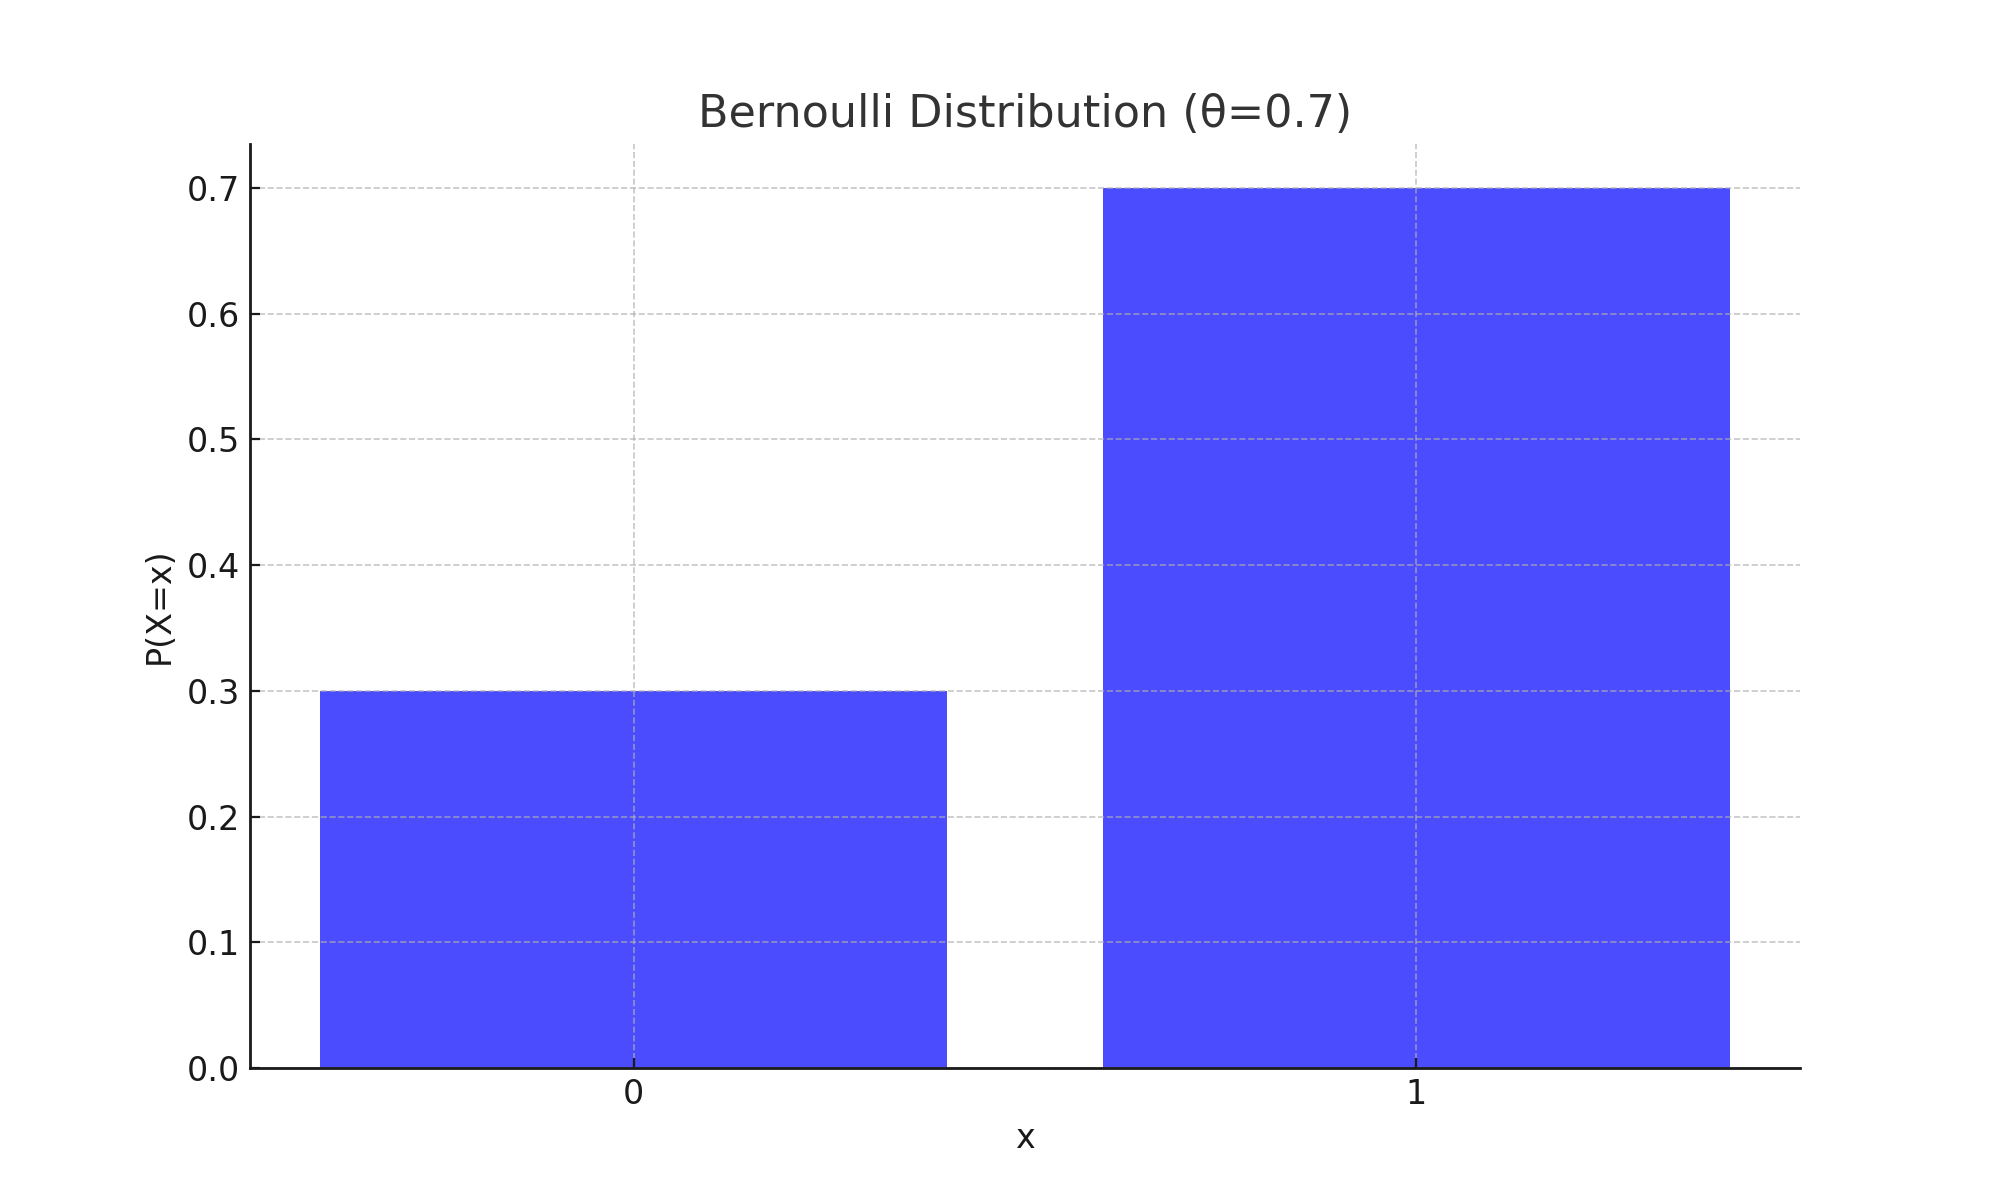
\includegraphics[width=\linewidth]{img/bernoulli_distribution.png}
    \caption{Bernoulli Distribution ($\theta=0.7$)}
    \label{fig:bernoulli}
\end{marginfigure}
This distribution underpins binary classification and models events like coin flips, where $\theta$ represents the success probability.

\subsection{Gaussian Distribution}




The \textbf{Gaussian distribution}, or normal distribution, models continuous data clustering around a mean. It is parameterised by the mean $\mu$ and variance $\sigma^2$. The probability density function (PDF) is:
\[
    f(x \mid \mu, \sigma^2) = \frac{1}{\sqrt{2\pi\sigma^2}} \exp\left(-\frac{(x - \mu)^2}{2\sigma^2}\right).
\]
\begin{marginfigure}
    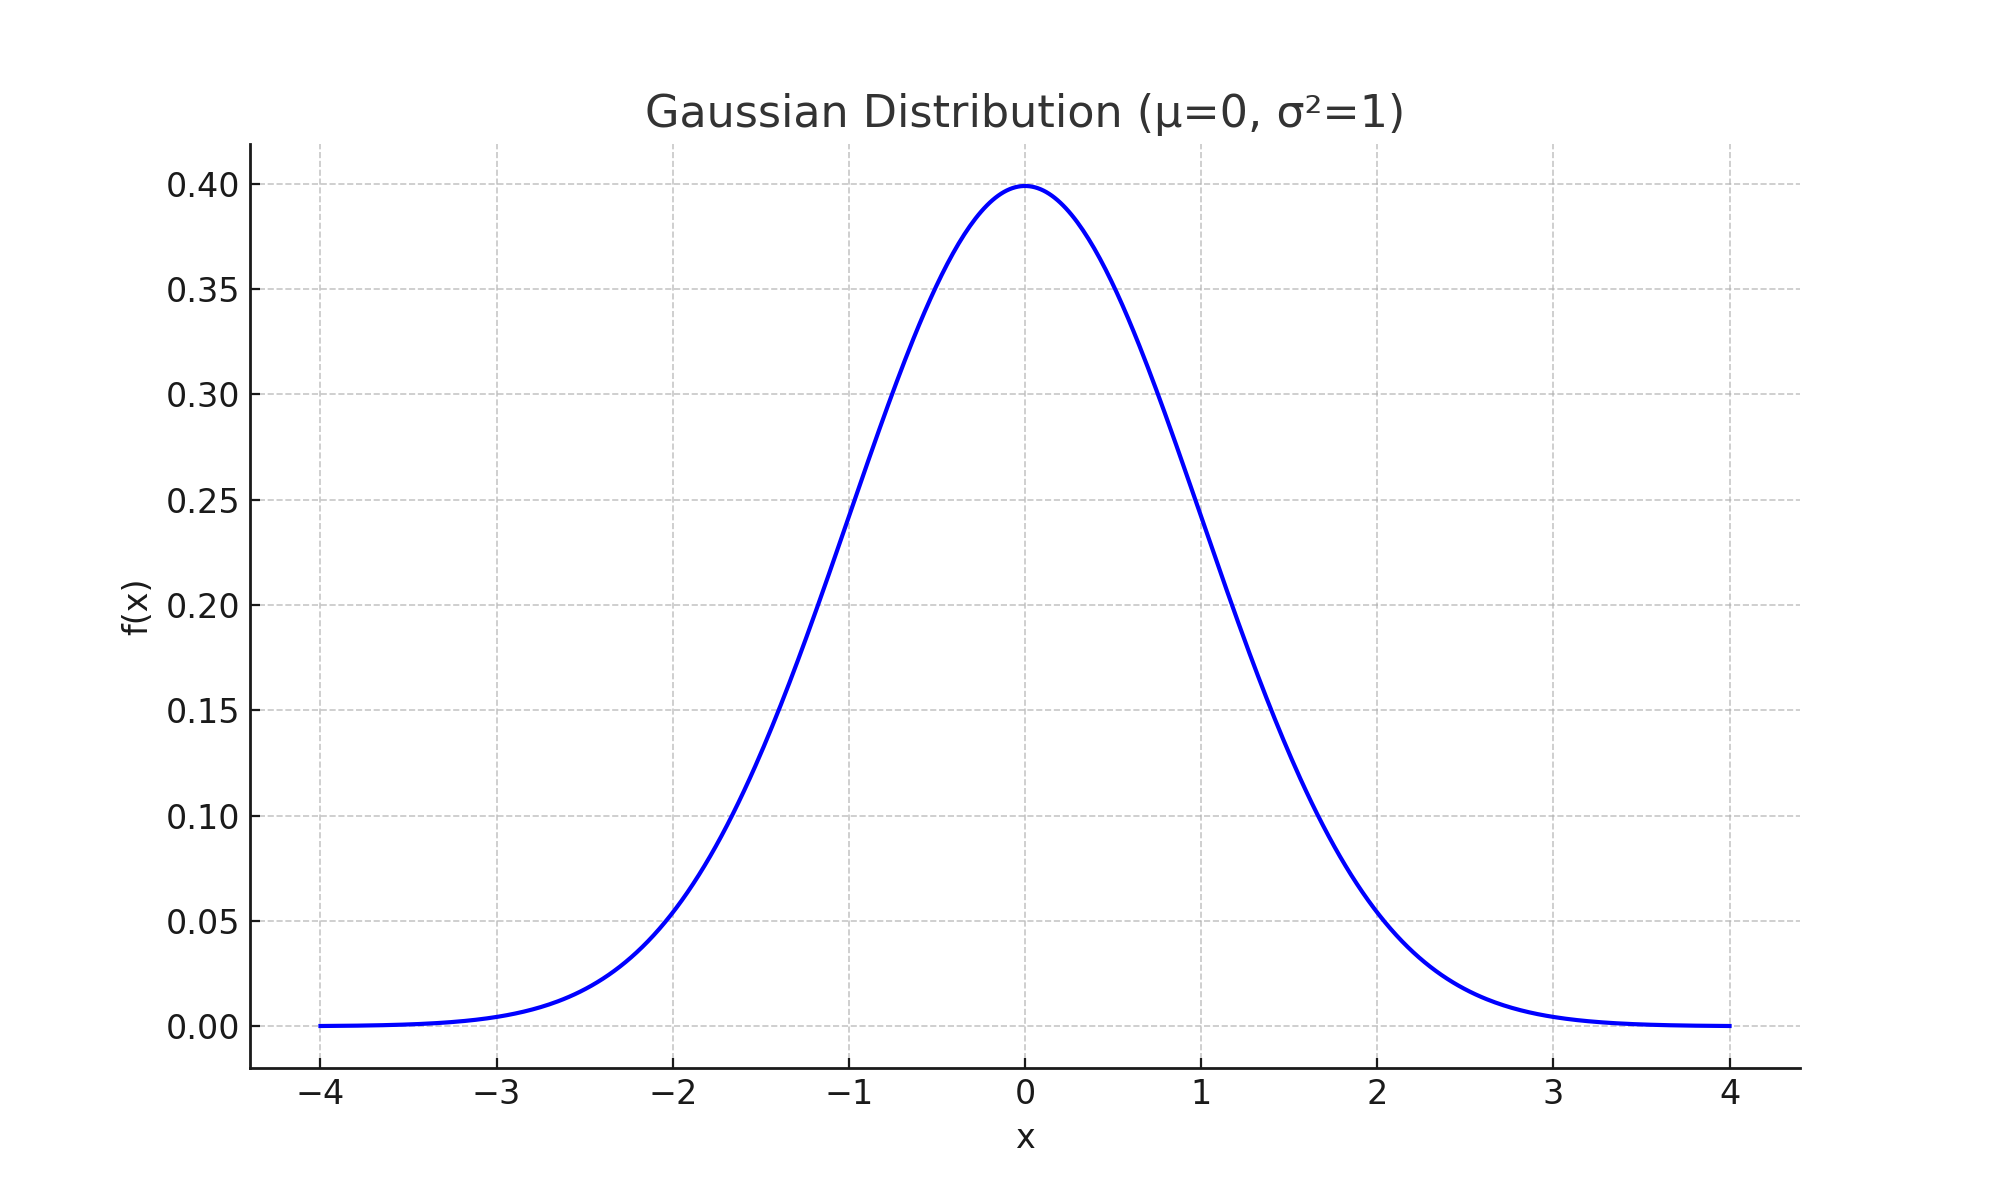
\includegraphics[width=\linewidth]{img/gaussian_distribution.png}
    \caption{Gaussian Distribution ($\mu=0, \sigma^2 = 1$)}
    \label{fig:gaussian}
\end{marginfigure}
The Gaussian distribution is fundamental in modelling natural phenomena and is a cornerstone for models like linear regression and Gaussian Naive Bayes.

\subsection{Beta Distribution}

The \textbf{Beta distribution} is a continuous distribution over $[0, 1]$, parameterised by shape parameters $\alpha$ and $\beta$. Its PDF is:
\[
    f(x \mid \alpha, \beta) = \frac{\Gamma(\alpha + \beta)}{\Gamma(\alpha) \Gamma(\beta)} x^{\alpha - 1} (1 - x)^{\beta - 1}, \quad 0 < x < 1,
\]
\begin{marginfigure}
    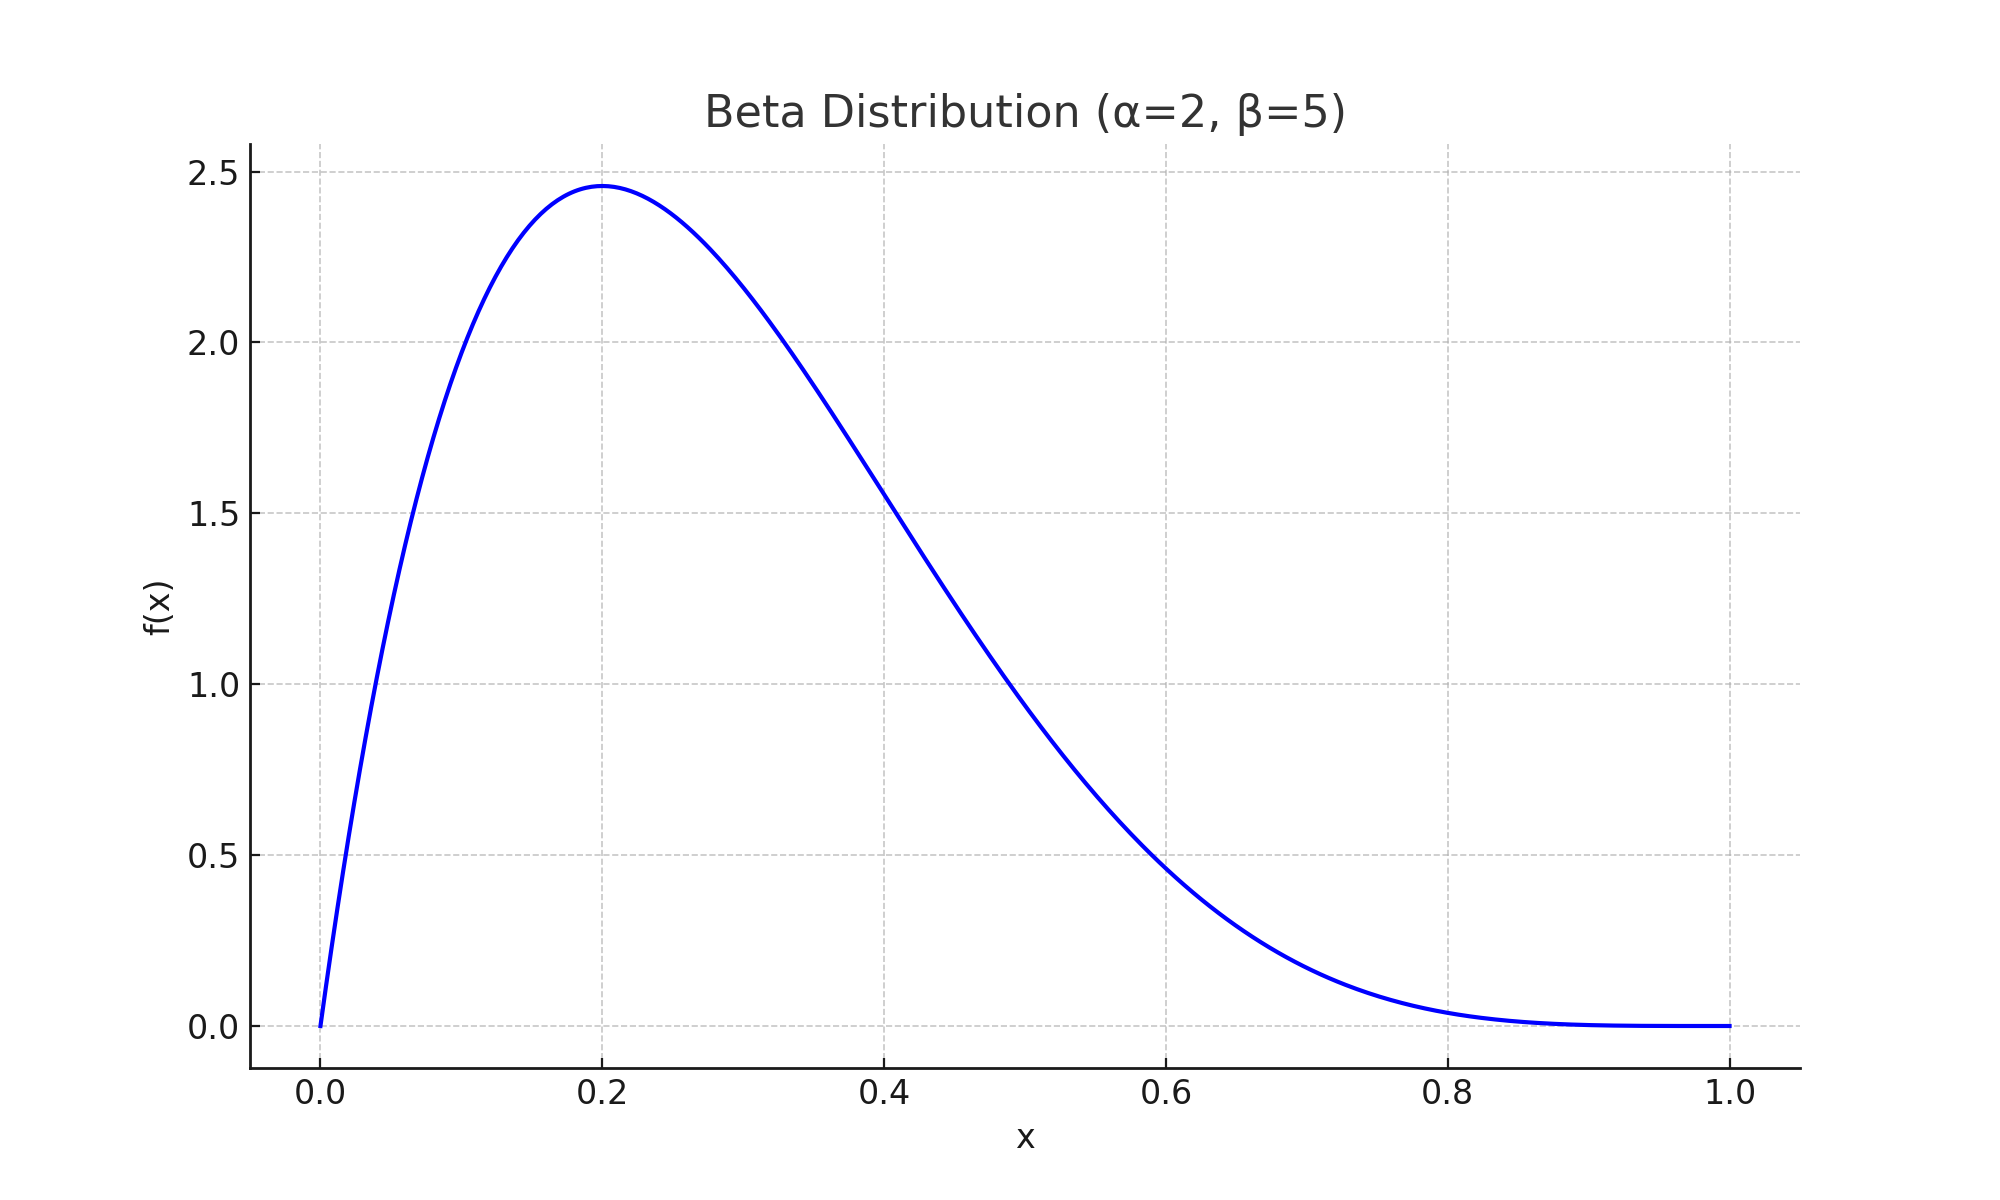
\includegraphics[width=\linewidth]{img/beta_distribution.png}
    \caption{Beta Distribution ($\alpha=2, \beta=5$)}
    \label{fig:beta}
\end{marginfigure}
where $\Gamma(\cdot)$ is the Gamma function. The Beta distribution is commonly used in Bayesian inference and modelling proportions due to its flexibility in shape.


\subsubsection{Beta Distribution: Mean}
\[
    \text{Mean} = \frac{\alpha}{\alpha + \beta}.
\]
The mean of the Beta distribution indicates the central tendency and depends on the relative magnitudes of \(\alpha\) and \(\beta\).

\subsubsection{Beta Distribution: Variance} \marginnote{
    \defsb{Gamma Function}{
        The Gamma function, denoted as $\Gamma(z)$, is a generalisation of the factorial to complex numbers. It is defined as:
        \[
            \Gamma(z) = \int_0^\infty t^{z-1} e^{-t} \, dt, \quad \text{for } z > 0.
        \]
        It satisfies the recurrence relation:
        \[
            \Gamma(z+1) = z \Gamma(z),
        \]
        with the special case $\Gamma(1) = 1$.

        \bigskip

        Note that for integers $\geq 1$, the gamma function reduces to the factorial: $\Gamma(n) = (n-1)!$ \bigskip

        For half-integers, odd $n$:

        \[
            \Gamma\left(\frac{n}{2}\right) = \frac{\sqrt{\pi}(n-2)!!}{2^{(n-1)/2}} 
        \]


    }

}
\[
    \text{Variance} = \frac{\alpha \beta}{(\alpha + \beta)^2 (\alpha + \beta + 1)}.
\]
The variance measures the spread of the distribution, with larger values of \(\alpha\) and \(\beta\) leading to a more concentrated distribution.





\subsubsection{Beta Distribution: Mode}
\[
    \text{Mode} = \frac{\alpha - 1}{\alpha + \beta - 2}, \quad \text{for } \alpha, \beta > 1.
\]
The mode gives the most likely value of the distribution. If either \(\alpha \leq 1\) or \(\beta \leq 1\), the mode is at the boundary (0 or 1, depending on the shape).

\subsubsection{Conjugacy in Bayesian Inference}

The Beta distribution is the \textit{conjugate prior} of the Binomial distribution. This means that if the likelihood function is Binomial, and the prior distribution is Beta, the posterior distribution is also Beta. Specifically, if the prior is \(\text{Beta}(\alpha, \beta)\) and the data consists of \(n_1\) successes and \(n_0\) failures, the posterior distribution is:
\[
    \text{Beta}(\alpha + n_1, \beta + n_0).
\]

The flexibility of the Beta distribution makes it a popular choice for modelling proportions, probabilities, and uncertainties over a fixed interval \([0, 1]\). \footnote{We will see more on this in the next two chapters.}


\subsection{Laplace Distribution}

The \textbf{Laplace distribution}, or double-exponential distribution, is characterised by a sharp peak at the mean and heavy tails. It is parameterised by the location parameter $\mu$ (mean) and scale parameter $b$. The PDF is:
\[
    f(x \mid \mu, b) = \frac{1}{2b} \exp\left(-\frac{|x - \mu|}{b}\right).
\]
\begin{marginfigure}
    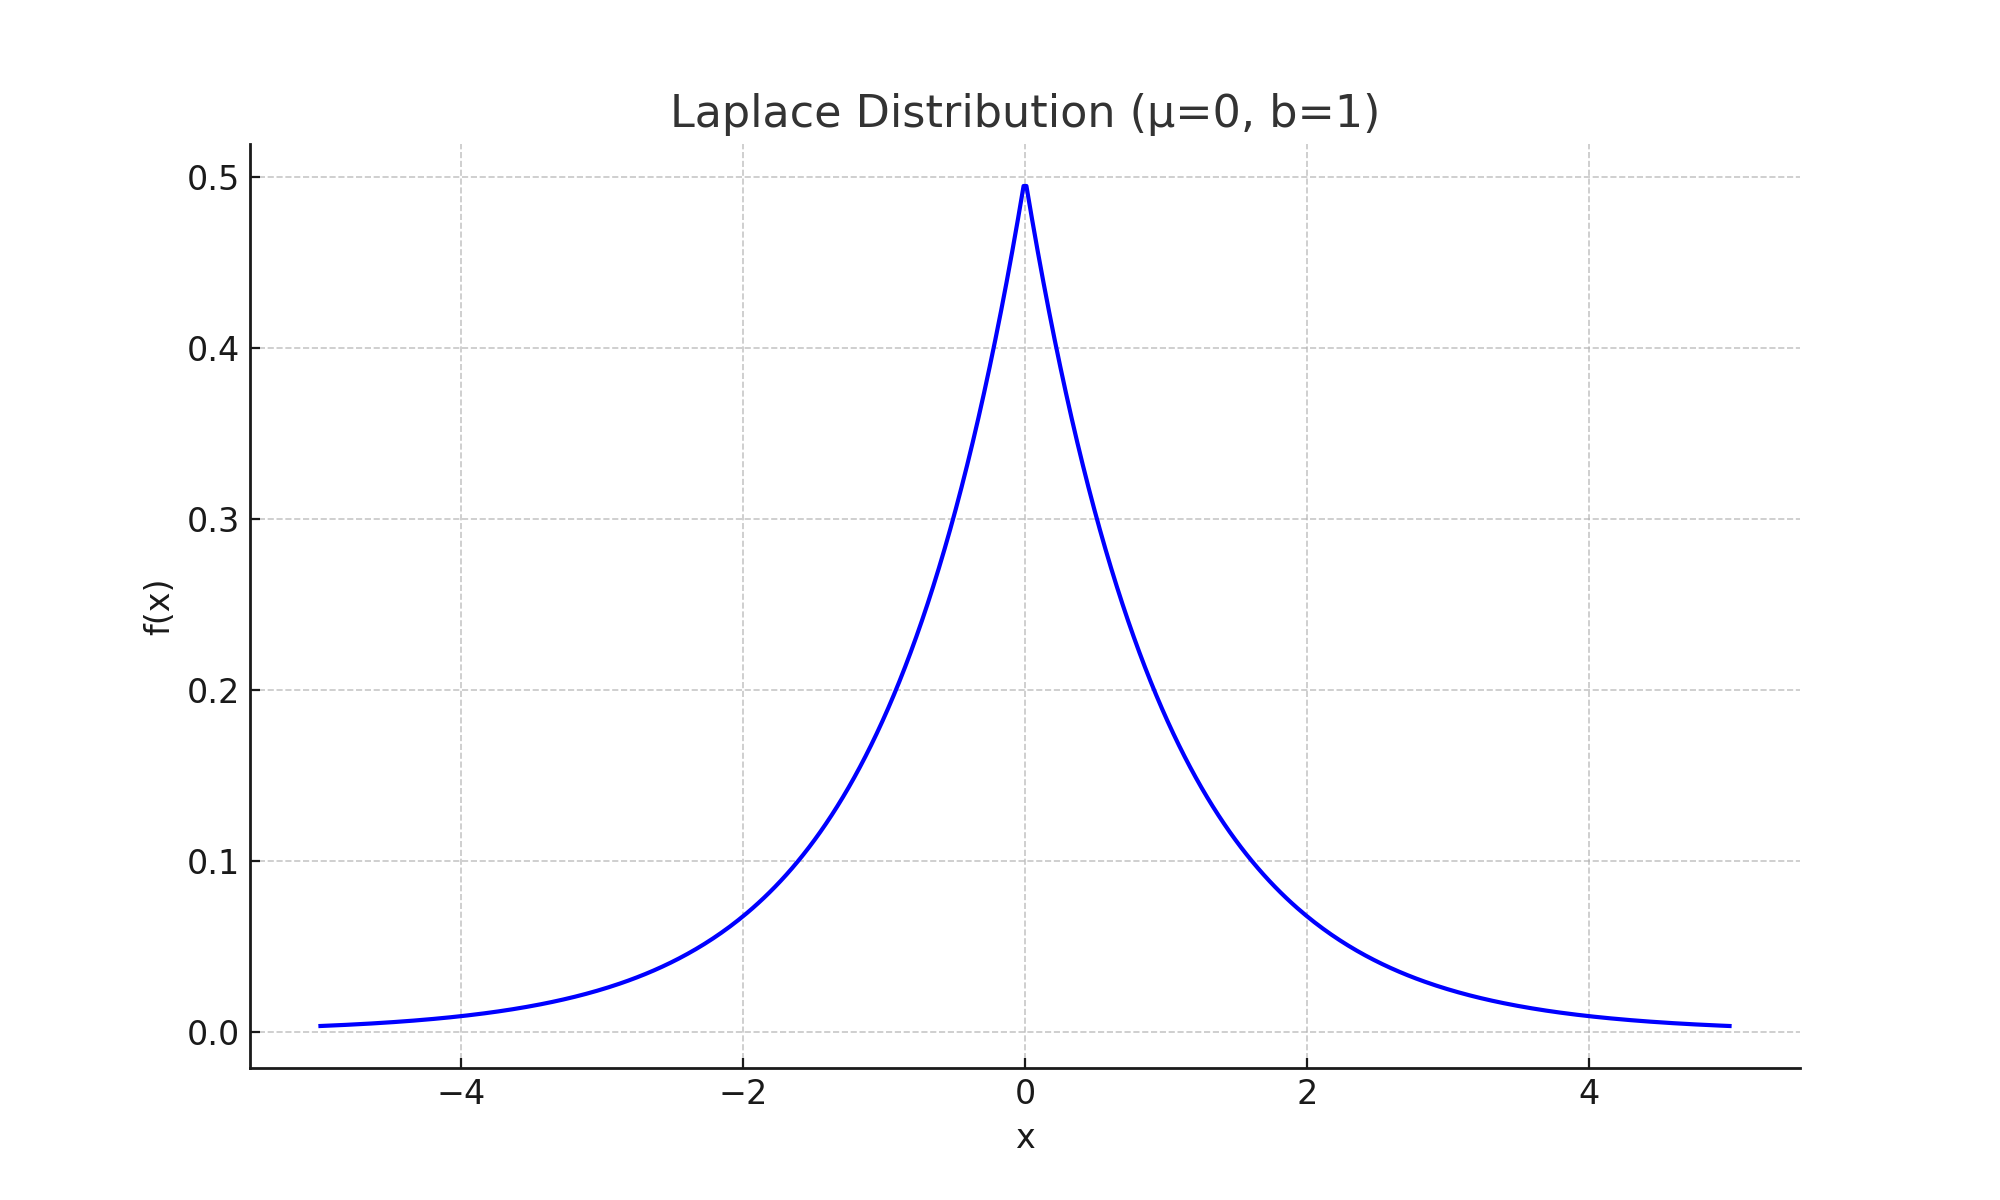
\includegraphics[width=\linewidth]{img/laplace_distribution.png}
    \caption{Laplace Distribution ($\mu=0, b=1$)}
    \label{fig:laplace}
\end{marginfigure}
This distribution is robust to outliers, making it useful in error modelling for robust regression and other contexts with large deviations from the mean.

\section{Multivariate Probability Distributions}

Multivariate probability distributions extend univariate distributions to multiple dimensions, capturing relationships between random variables. This section covers key examples with detailed mathematical expressions.

\subsection{Multinoulli Distribution}


The \textbf{Multinoulli distribution}, or categorical distribution, generalises the Bernoulli distribution to handle $k$ discrete outcomes. It is parameterised by a vector of probabilities $\boldsymbol{\theta} = [\theta_1, \theta_2, \ldots, \theta_k]$, where $\theta_i$ is the probability of observing the $i$-th category, with:
\[
    \sum_{i=1}^k \theta_i = 1 \quad \text{and } \theta_i \geq 0 \, \forall i.
\]
\begin{marginfigure}
    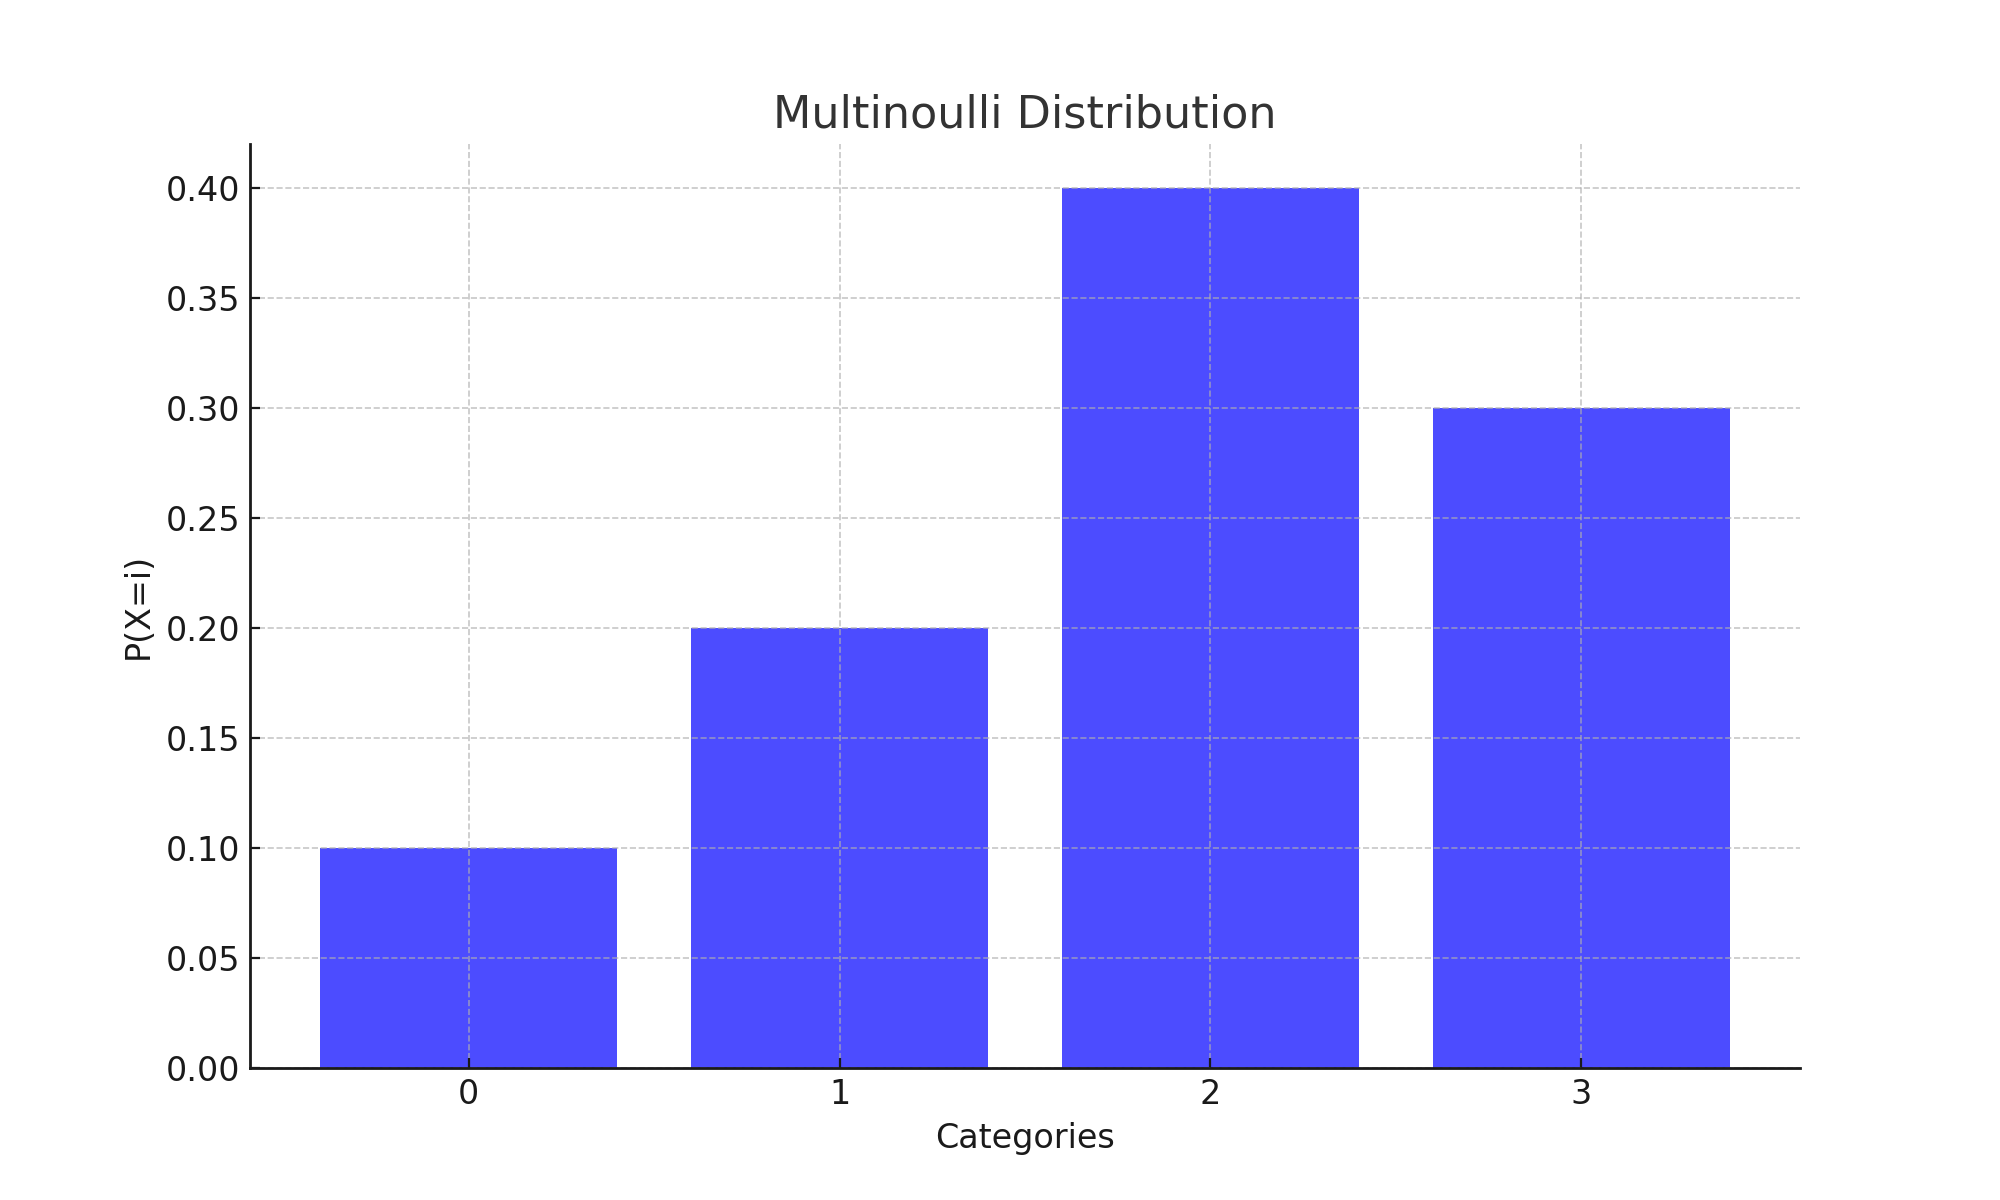
\includegraphics[width=\linewidth]{img/multinoulli_distribution.png}
    \caption{Multinoulli Distribution}
    \label{fig:multinoulli}
\end{marginfigure}

The probability mass function (PMF) of a Multinoulli random variable $X$ is:
\[
    P(X = i) = \theta_i, \quad i = 1, 2, \ldots, k.
\]

\sn{}{\raggedright
    The Multinoulli distribution is commonly used in classification tasks to model probabilities across categories. For $k = 2$, it reduces to the Bernoulli distribution.}

\subsection{Multivariate Gaussian Distribution}


The \textbf{Multivariate Gaussian distribution} generalises the Gaussian distribution to $n$ dimensions, modelling continuous data with interdependencies between variables. It is parameterised by:
\begin{itemize}
    \item \textbf{Mean vector:} $\boldsymbol{\mu} = [\mu_1, \mu_2, \ldots, \mu_n]^\top$, where $\mu_i$ is the mean of the $i$-th variable.
    \item \textbf{Covariance matrix:} $\boldsymbol{\Sigma}$, an $n \times n$ positive semi-definite matrix, encoding variances and covariances:
          \[
              \Sigma_{ij} = \mathbb{E}[(X_i - \mu_i)(X_j - \mu_j)].
          \]
\end{itemize}

\begin{marginfigure}
    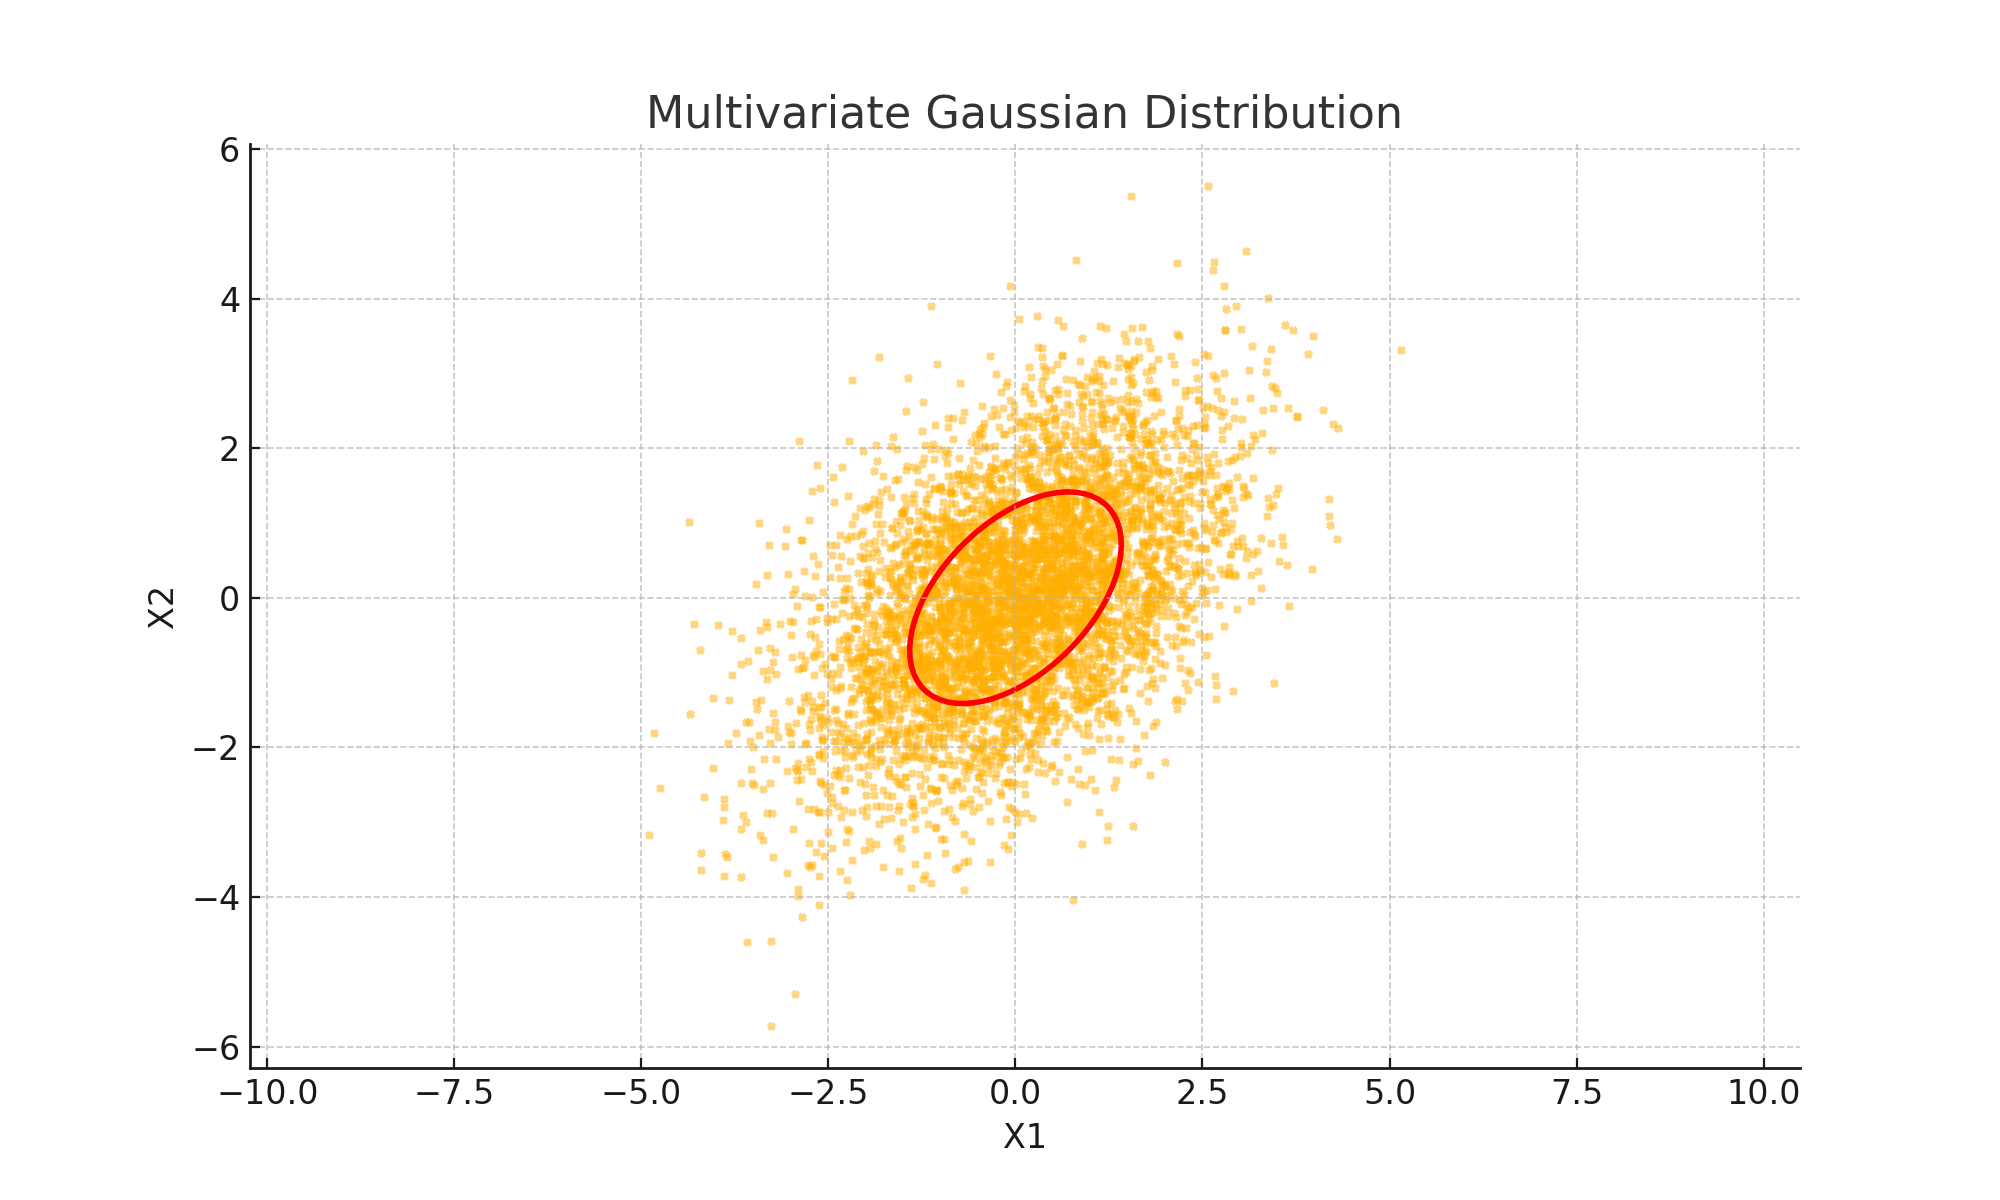
\includegraphics[width=\linewidth]{img/multivariate_gaussian_distribution.png}
    \caption{Visualisation of a Multivariate Gaussian Distribution with mean vector \([0, 0]\) and covariance matrix \(\begin{bmatrix} 2 & 1 \\ 1 & 2 \end{bmatrix}\). The confidence ellipse represents one standard deviation.}
    \label{fig:multivariate_gaussian}
\end{marginfigure}

The probability density function (PDF) is:
\[
    f(\mathbf{x} \mid \boldsymbol{\mu}, \boldsymbol{\Sigma}) = \frac{1}{(2\pi)^{n/2} |\boldsymbol{\Sigma}|^{1/2}}
    \exp\left(-\frac{1}{2} (\mathbf{x} - \boldsymbol{\mu})^\top \boldsymbol{\Sigma}^{-1} (\mathbf{x} - \boldsymbol{\mu})\right),
\]
where $\mathbf{x} = [x_1, x_2, \ldots, x_n]^\top$ is the random vector, and $|\boldsymbol{\Sigma}|$ denotes the determinant of $\boldsymbol{\Sigma}$.

\paragraph{Geometric Interpretation:}
In two dimensions, the Multivariate Gaussian distribution is visualised as an ellipse centered at $\boldsymbol{\mu}$. The covariance matrix $\boldsymbol{\Sigma}$ determines the orientation and spread:
\begin{itemize}
    \item Eigenvalues $\lambda_1$ and $\lambda_2$ of $\boldsymbol{\Sigma}$ represent the variances along the ellipse's principal axes.
    \item Eigenvectors $\mathbf{v}_1$ and $\mathbf{v}_2$ determine the directions of the principal axes.
    \item The lengths of the axes are $\sqrt{\lambda_1}$ and $\sqrt{\lambda_2}$.
\end{itemize}

\sn{}{This geometric insight generalises to higher dimensions, where $\boldsymbol{\Sigma}$ determines the spread and orientation of the distribution in $n$-dimensional space.}

\subsection{Multivariate Laplace Distribution}
The Multivariate Gaussian is widely used in applications such as:
\begin{itemize}
    \item Clustering algorithms (e.g., Gaussian Mixture Models).
    \item Dimensionality reduction (e.g., Principal Component Analysis).
    \item Probabilistic modelling of multivariate data.
\end{itemize}
\begin{marginfigure}
    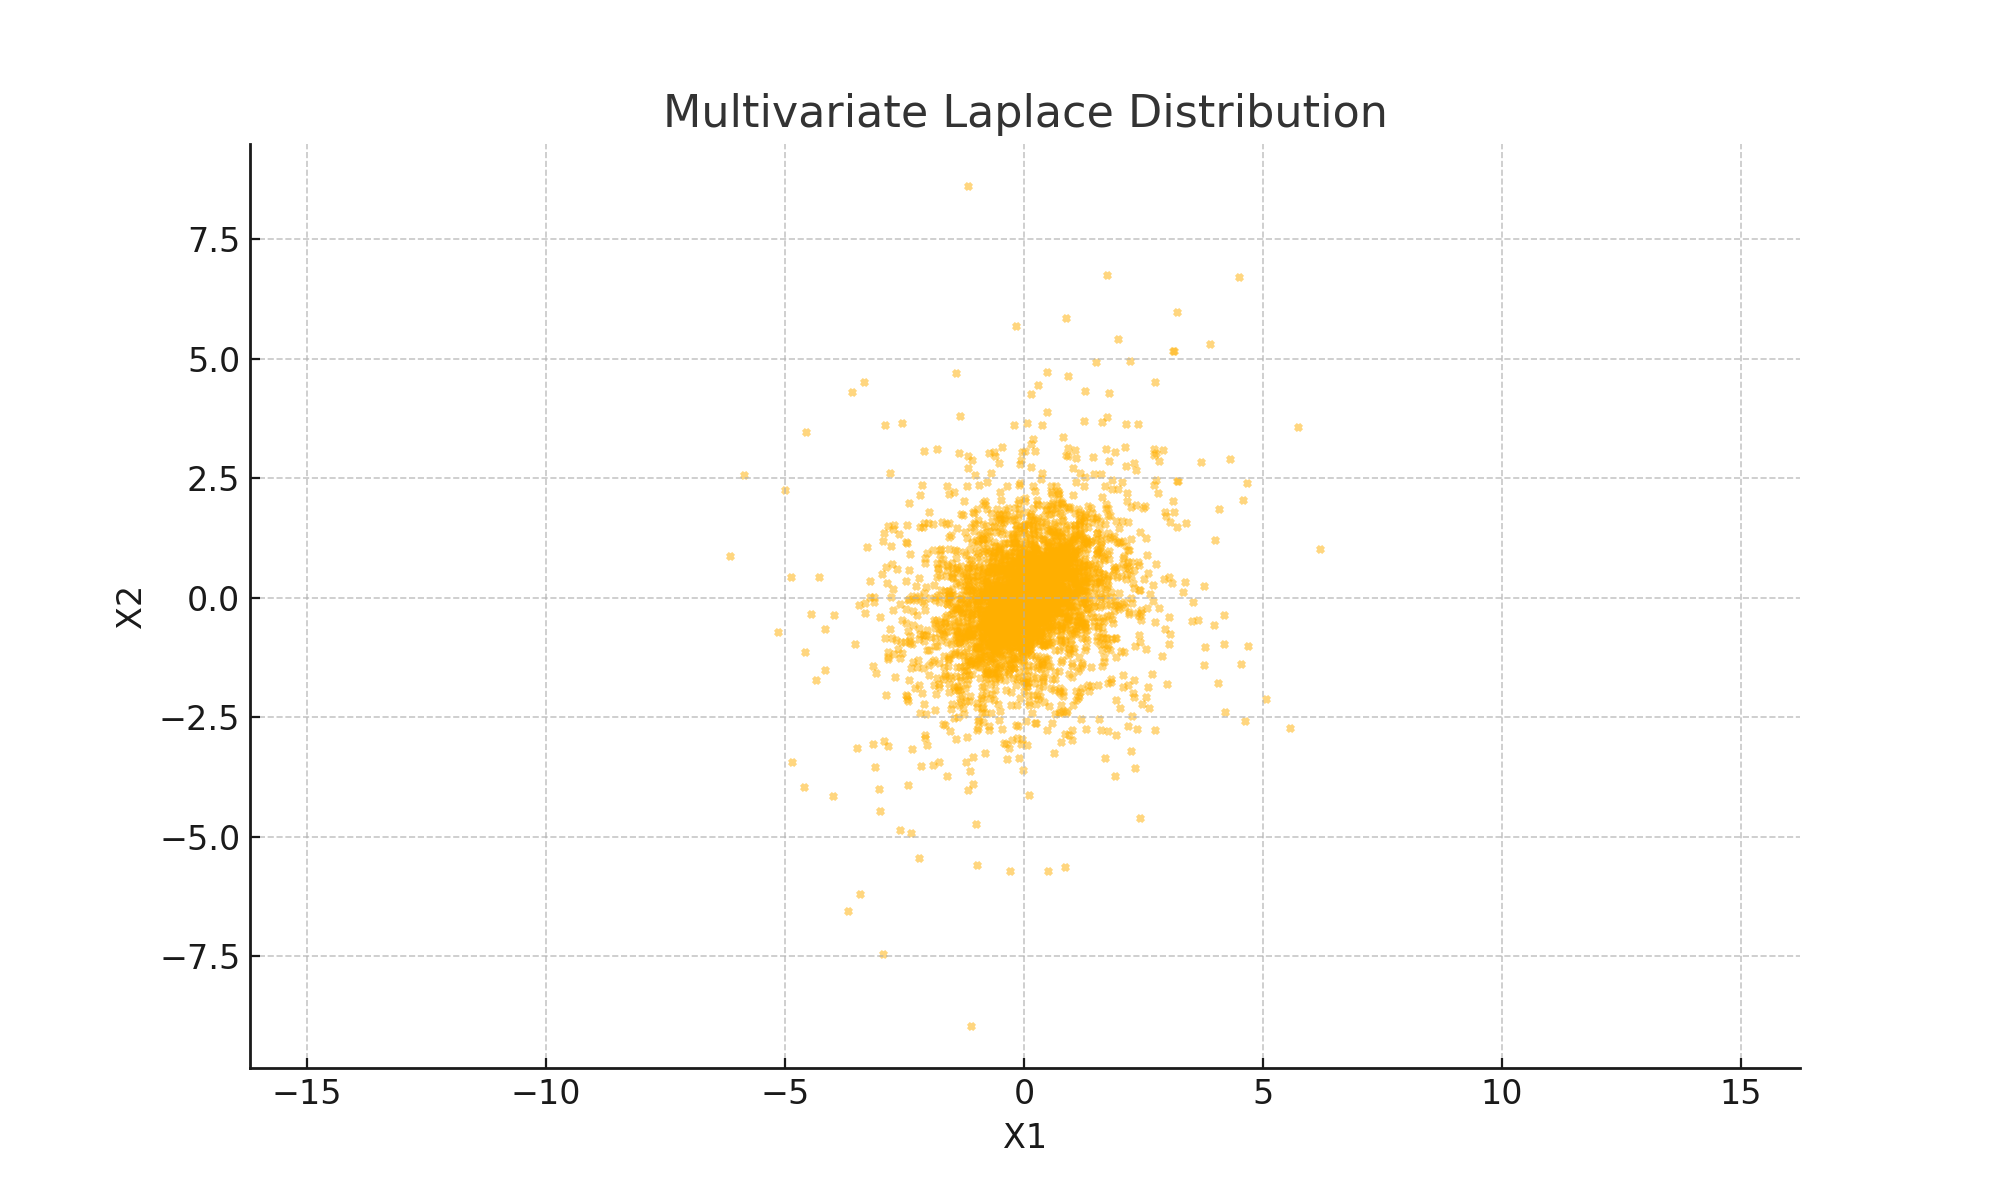
\includegraphics[width=\linewidth]{img/multivariate_laplace_distribution.png}
    \caption{Visualisation of a Multivariate Laplace Distribution with mean vector \([0, 0]\) and covariance matrix \(\begin{bmatrix} 2 & 1 \\ 1 & 2 \end{bmatrix}\). Samples highlight heavy tails and sharp peaks characteristic of the Laplace distribution.}
    \label{fig:multivariate_laplace}
\end{marginfigure}



The \textbf{Multivariate Laplace distribution} extends the univariate Laplace distribution to $n$ dimensions. It is useful for robust modelling due to its heavier tails, which provide resistance to outliers. This distribution is parameterised by:
\begin{itemize}
    \item \textbf{Mean vector:} $\boldsymbol{\mu}$, representing the central location.
    \item \textbf{Covariance matrix:} $\boldsymbol{\Sigma}$, which determines scale and spread.
\end{itemize}

The probability density function (PDF) is:
\[
    f(\mathbf{x} \mid \boldsymbol{\mu}, \boldsymbol{\Sigma}) = \frac{2}{(2\pi)^{n/2} |\boldsymbol{\Sigma}|^{1/2}}
    \frac{1}{\sqrt{(\mathbf{x} - \boldsymbol{\mu})^\top \boldsymbol{\Sigma}^{-1} (\mathbf{x} - \boldsymbol{\mu})}}
    \exp\left(-\sqrt{(\mathbf{x} - \boldsymbol{\mu})^\top \boldsymbol{\Sigma}^{-1} (\mathbf{x} - \boldsymbol{\mu})}\right),
\]
where $\mathbf{x}$ is the random vector, and $\boldsymbol{\Sigma}$ defines the covariance structure.

\sn{}{The Multivariate Laplace distribution is often used in:
    \begin{itemize}
        \item Robust regression, where heavy tails help reduce sensitivity to outliers.
        \item Error modelling in contexts requiring robustness.
    \end{itemize}}


\section{Common Conjugate Priors}
\begin{table*}[h!]
\centering
\begin{tabular*}{\textwidth}{@{\extracolsep{\fill}}lll@{}}
    \toprule
    \textbf{Likelihood}                  & \textbf{Prior (Conjugate)} & \textbf{Posterior}     \\ \midrule
    Bernoulli/Binomial                   & Beta                       & Beta                   \\
    Poisson                              & Gamma                      & Gamma                  \\
    Gaussian (Known Variance)            & Gaussian                   & Gaussian               \\
    Gaussian (Unknown Variance)          & Normal-Inverse-Gamma       & Normal-Inverse-Gamma   \\
    Gaussian (Unknown Mean and Variance) & Normal-Inverse-Wishart     & Normal-Inverse-Wishart \\
    Multinomial                          & Dirichlet                  & Dirichlet              \\
    Exponential                          & Gamma                      & Gamma                  \\
    Negative Binomial                    & Beta                       & Beta                   \\
    Categorical                          & Dirichlet                  & Dirichlet              \\
    \bottomrule
\end{tabular*}
\vspace{3em}
\caption{Common Conjugate Priors in Bayesian Inference}
\label{tab:conjugate_priors}
\end{table*}
